\documentclass[12pt]{article}
\usepackage{tikz}
\usepackage{geometry}

\usetikzlibrary{mindmap}

\author{ supercentinel }
%2019-01-01
\geometry{landscape, margin=1cm}

\begin{document}
\begin{center}
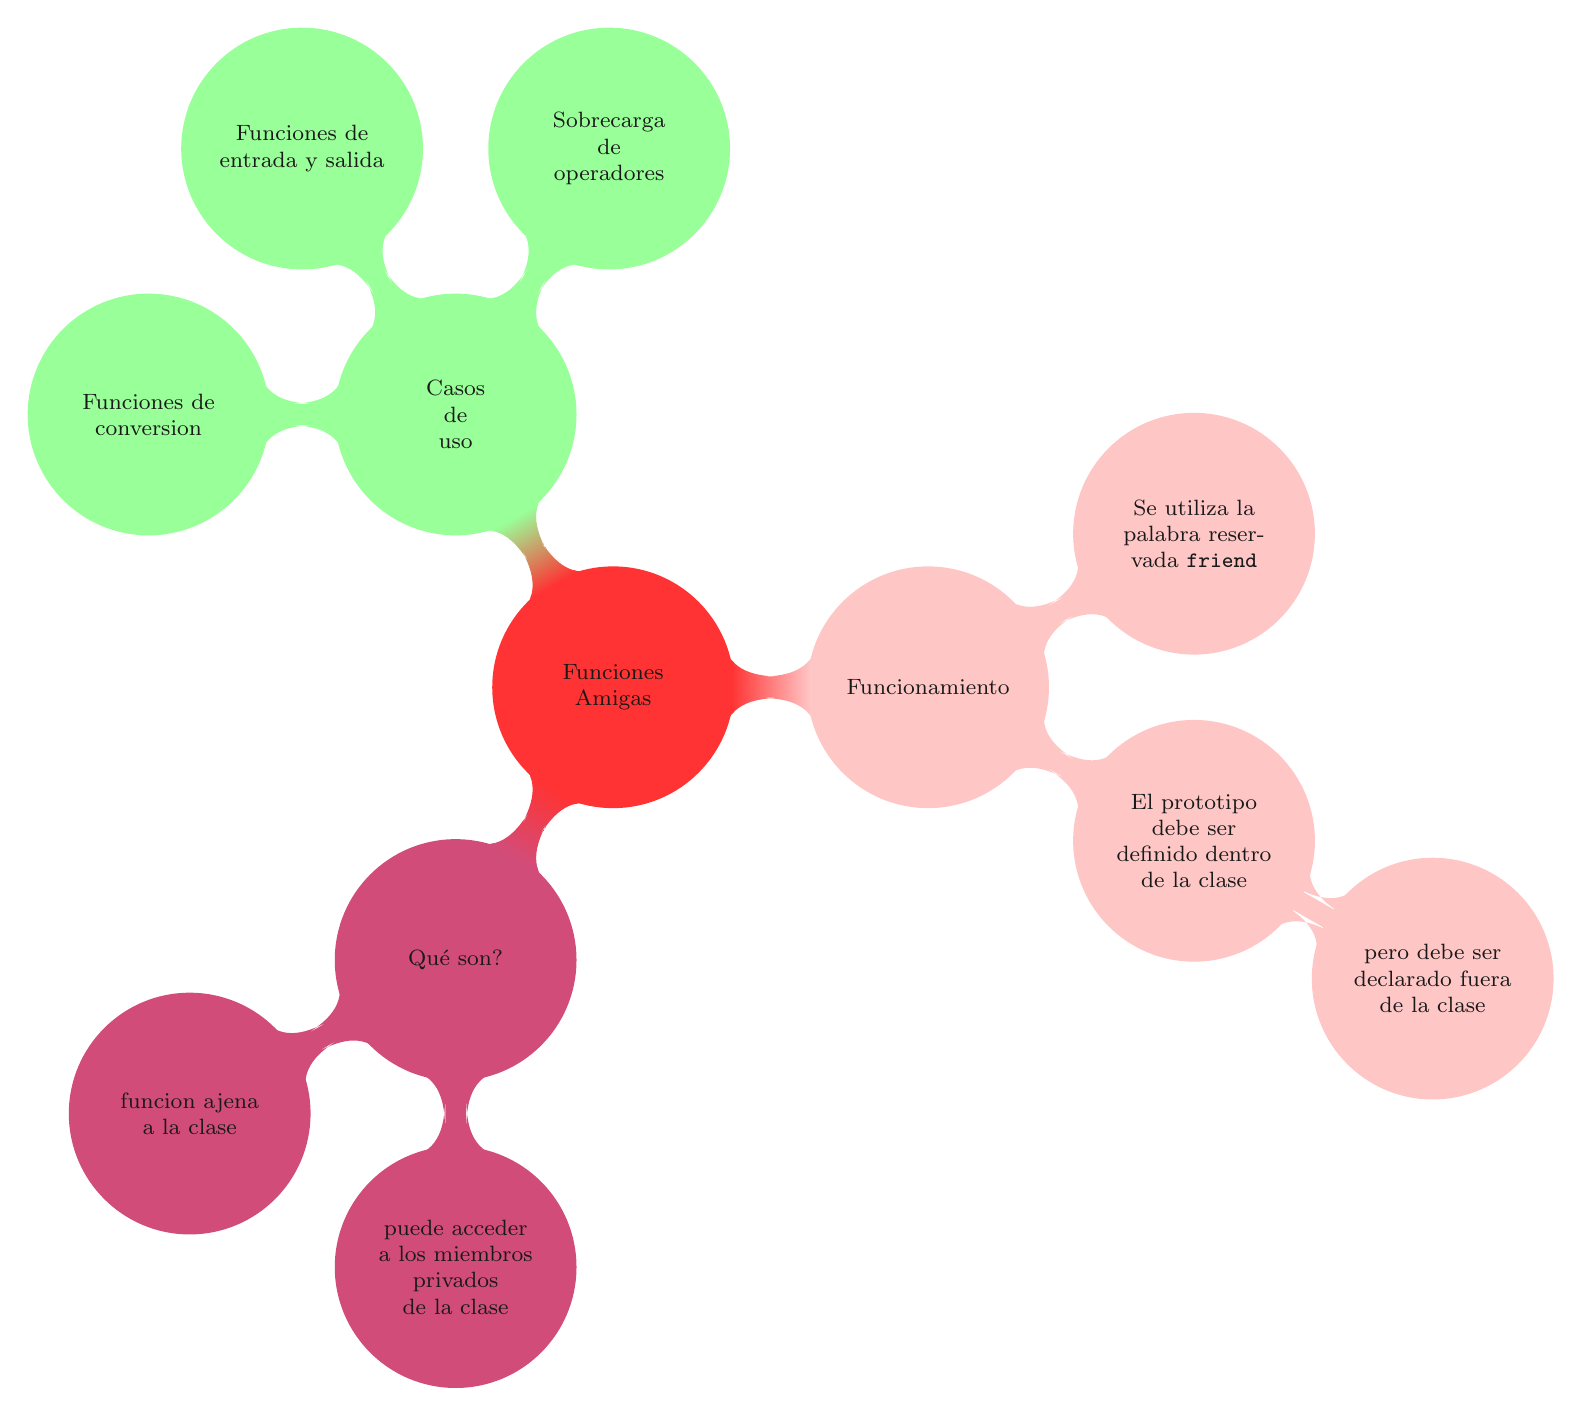
\begin{tikzpicture}[small mindmap, grow cyclic, every node/.style=concept, concept color=red!80, text=black!90, minimum size=3.0cm,
    level 1/.style={level distance=4.5cm,sibling angle=360/3},
    level 1/.style={level distance=4.0cm,sibling angle=360/3},
    level 2/.style={level distance=3.9cm,sibling angle=60},
    level 3/.style={level distance=3.5cm,sibling angle=60},
    ]
    \node{ Funciones Amigas }
    child[concept color=purple!70] { node { Qué son? }
        child { node { funcion ajena a la clase } }
        child { node { puede acceder a los miembros privados de la clase } }
    }
    child[concept color=pink!90] { node { Funcionamiento }
        child { node { El prototipo debe ser definido dentro de la clase }
            child { node { pero debe ser declarado fuera de la clase } }
        }
        child { node { Se utiliza la palabra reservada \texttt{friend} } }
    }
    child[concept color=green!40] { node { Casos\\de\\uso }
        child { node { Sobrecarga\\de\\operadores } }
        child { node { Funciones de entrada y salida } }
        child { node { Funciones de conversion } }
    }
    ;
\end{tikzpicture}
\end{center}
\end{document}
